\documentclass[]{article}
\usepackage{amsmath}
\usepackage{graphicx}
\usepackage{listings}

\usepackage{color}
%
%\usepackage{enumitem}
%\setlist[itemize]{leftmargin=*}
%\setlist[enumerate]{leftmargin=*}

\definecolor{dkblue}{rgb}{0.6,0.0,0}
\definecolor{gray}{rgb}{0.5,0.5,0.5}
%\definecolor{yellow}{rgb}{0.0,0.5,0.5}

\lstset{frame=tb,
  language=bash,
  aboveskip=3mm,
  belowskip=3mm,
  showstringspaces=false,
  columns=flexible,
  basicstyle={\small\ttfamily},
  numbers=none,
  breaklines=true,
  breakatwhitespace=true,
  tabsize=4
}

\begin{document}

\title{A Cosmology Calculator }
\maketitle

\noindent The propose of the program is to provide some of the more commonly used cosmological parameters, as a function of redshift. The parameters provided are the comoving distance, $r$, the luminosity distance, $D_\mathrm{L}$, the angular diameter distance $D_\mathrm{A}$ and the age of the universe at redshift $z$, $t_\mathrm{age}$. \\

\noindent If you're in astro, this will be a program you will almost certainly use at some point. If you're not in astro, it will at least be a simple program for you to use to learn python. \\

\noindent These notes are in no way intended to give you a full understanding of the parameters and their meaning, or derivation. They give a general introduction to the theory for those interested, and provide the maths you need to write a cosmology calculator. If you are not interested in the theory, it is entirely possible to just use the maths in boxes in these notes to write the code, without even understanding it. If this is you, note these equations down, and skip to Section~\ref{sec:code}. If you are interested in astro however you can read the notes to understand what you are computing. For a more thorough run down of the cosmology, and a full understanding of the derivation and significance of these parameters, I recommend Stuart Wyithe and Bart Pindor's Cosmology Notes for the Masters Cosmology Course, in particular chapters 2 though to 10. \\

\section{The cosmology}

\noindent I will explain each of the parameters to be computed below, but first I need to introduce the Friedman Equation and some other things.\\

\noindent The metric used to describe the universe is called the Robertson-Walker Metric. An description of the features of this metric, and an explanation of why it is used is not included here. See the aforementioned Masters Cosmology notes for more information. The Friedman Model is a solution to the Robertson-Walker Metric, which can be derived from Einstein’s Equations.\\

\noindent From the Friedman model one can obtain an expression for the time rate of change of the \itshape scale factor\upshape, $a$
\begin{equation}
H = \frac{\dot a}{a}.
\end{equation}
The scale factor describes how big space is at time $t$. Computing the derivative in this equation yields
\begin{equation}
H(z)^2 = H_0^2[\Omega_\mathrm{m} a^{-3}+\Omega_\mathrm{R} a^{-4}+\Omega_\Lambda],
\end{equation}
\noindent where $\Omega_\mathrm{m}$ is the density of mass in the universe, $\Omega_\mathrm{R}$ is the density of radiation in the universe, and $\Omega_\Lambda$ is the dark energy density. This equation is called the Friedman Equation. Note that here and throughout this document $\Omega_\mathrm{R}$ is explicitly included for completeness, however in the calculator code (and in general in Astrophysics), it is assumed to be zero for all redshifts below $z\sim1000$. This is because it goes as $a^{-4}$ and $a$ goes to infinity at low redshifts, so the contribution from this term becomes negligible at smaller redshifts. The scale factor can be written in terms of the redshift, since light is being redshifted in space by the size of space changing
\begin{equation}
a = \frac{1}{(1+z)}.
\end{equation}
The Friedman equation gives the evolution of the Hubble parameter with redshift for a given \itshape cosmology~\upshape (here ‘cosmology’ refers to the choice of $\Omega_\mathrm{m}$, $\Omega_\mathrm{R}$ and $\Omega_\Lambda$). The Hubble \itshape constant\upshape , which you may be familiar with, doesn't take into account the evolution of the universe. It gives the expansion of the universe \itshape today~\upshape at redshift 0. The way the expansion of the universe evolves with redshift is encapsulated by the terms in the square brackets in the Friedman equation above. 

\noindent Note that redshift doesn't get larger with time, it gets larger the further \itshape back~\upshape in time you go, and is zero now. In other words it is defined to be zero at the present, and to be infinite at the big bang. This makes sense when you think about what redshift means. Redshift gives the fractional shift in the wavelength of light emitted at some time in the past, relative to how we see it now. So it makes sense that something emitted now will have a redshift of 0 because it hasn't had its wavelength shifted at all. The further back you look (which is equivalent to saying the further away you look), the more the wavelength of the light has been stretched (i.e. redshifted) due to the expansion of the universe. \\

\noindent A characteristic scale in cosmology is the \itshape Hubble distance~\upshape, $d_H$. This is the size of the observable universe at a given redshift,
\begin{equation}
d_H = \frac{c}{H(z)}.
\end{equation}
Another way of thinking of this is that the Hubble distance is the distance between the Earth and the galaxies which are currently receding from us at the speed of light (i.e. things which are just now becoming invisible to us because their light can never reach us). \\

\noindent We now have what we need to get the comoving distance.

\subsection{Comoving distance (or proper distance)}

This is the distance to an object in \itshape comoving~\upshape coordinates. That is, this distance takes the expansion of the universe into account. \\

\noindent The comoving distance is obtained by integrating the Hubble distance from the redshift in question to now (so from redshift $z$ to redshift 0)
\begin{equation}
r_\mathrm{com} = \int_0^z d_H \mathrm{d}z,
\end{equation}
or expanding
\begin{equation}
\boxed{
\begin{split}
r_\mathrm{com} &= c\int_0^z \frac{1}{H(z)}\mathrm{d}z\\
&= \frac{c}{H_0}\int_0^z [\Omega_\mathrm{m} (1+z)^{3}+\Omega_\mathrm{R} (1+z)^{4}+\Omega_\Lambda]^{-1/2}\mathrm{d}z
\end{split}
}
\end{equation}\\

\noindent A diagram of the comoving distance is shown in the first panel of Figure~\ref{fig:distances}.

\subsection{Luminosity distance}

As you no doubt know, flux falls off as radius squared. If you know the intrinsic brightness of something, this can be used measure the distance to it. In an expanding universe however, the amount of space for the light to propagate through is increasing, and so it’s no longer as simple as radius squared. \\

\noindent The luminosity of an object observed at Earth, in terms of it’s emitted flux is 
\begin{equation}
L_\mathrm{obs} = L_\mathrm{em}a^2
\end{equation}
or
\begin{equation}
L_\mathrm{obs} = \frac{L_\mathrm{em}}{(1+z)^2},
\end{equation}
where one factor of $a$ is due to time dilation (photons lose energy…), and one is due to red shift (…and they arrive at a lower rate).\\

\noindent The distance one would measure in a static universe is
\begin{equation}
d_\mathrm{L} = \sqrt{\frac{L_\mathrm{em}}{4\pi F_\mathrm{obs}}},
\end{equation}
and 
\begin{equation}
F_\mathrm{obs} = \frac{L_\mathrm{obs}}{4\pi r^2}.
\end{equation}
Combining these, one can write the luminosity distance in terms of redshift
\begin{equation}
\boxed{D_\mathrm{L} = \frac{r_\mathrm{com}}{a} = r_\mathrm{com} (1+z)}
\end{equation}
So you can see that once you have the comoving distance, getting the luminosity distance is trivial! \\

\noindent A diagram of the luminosity distance is shown in the second panel of Figure~\ref{fig:distances}.

\subsection{Angular diameter distance}
This is the distance according to the angular size of an object on the sky, compared to some known size.\\ 

\noindent When you look at a 30 cm ruler at a distance, it has a certain angular size, that is, it subtends some angle in your vision. For very distant objects which have a small angular size (like a galaxy in the night sky), you can use the \itshape small angle approximation~\upshape to relate the angular size of the object to the true size and the distance to the object
\begin{equation}
d \approx R \theta,
\end{equation}
where $\theta$ is the angular size of an object, $d$ is the true size of the object and $R$ is the distance to the object. If $d$ and $theta$ are known, then the distance to an object can be obtained using this relation. \\

\noindent This is all assuming that the lines from the edges of the object to the observer are straight, so that you can use trigonometry in the normal way. But the way we determine the location of the edges of an object is from the light coming from it, and in an expanding universe these are no longer straight. \\

\noindent If we consider two points separated by some apparent angular separation $\theta$, at a distance of $R$, the light from these two points will travel along curved null geodesics to reach us, and so the angle of incidence of the light will not the the same as the angle of emission. This is like the way lenses can create apparent images, because they alter the angle of incidence of the light rays from a source on our eyes. \\

\noindent To account for this, we need to re-define the edges of the small angle triangle, and take the expansion of the universe into account. The apparent distance with expansion will be the comoving distance, multiplied by $a$, the scale factor. 
\begin{equation}
\boxed{D_\mathrm{A} = r_\mathrm{com} a = \frac{r_\mathrm{com}}{1+z}}
\end{equation}
This is the angular diameter distance, and as with the luminosity distance, getting the it is trivial once you have the comoving distance. \\

\noindent A diagram of the angular diameter distance is shown in the third panel of Figure~\ref{fig:distances}.

\begin{figure*}[h!]
\hspace*{-2.7cm}
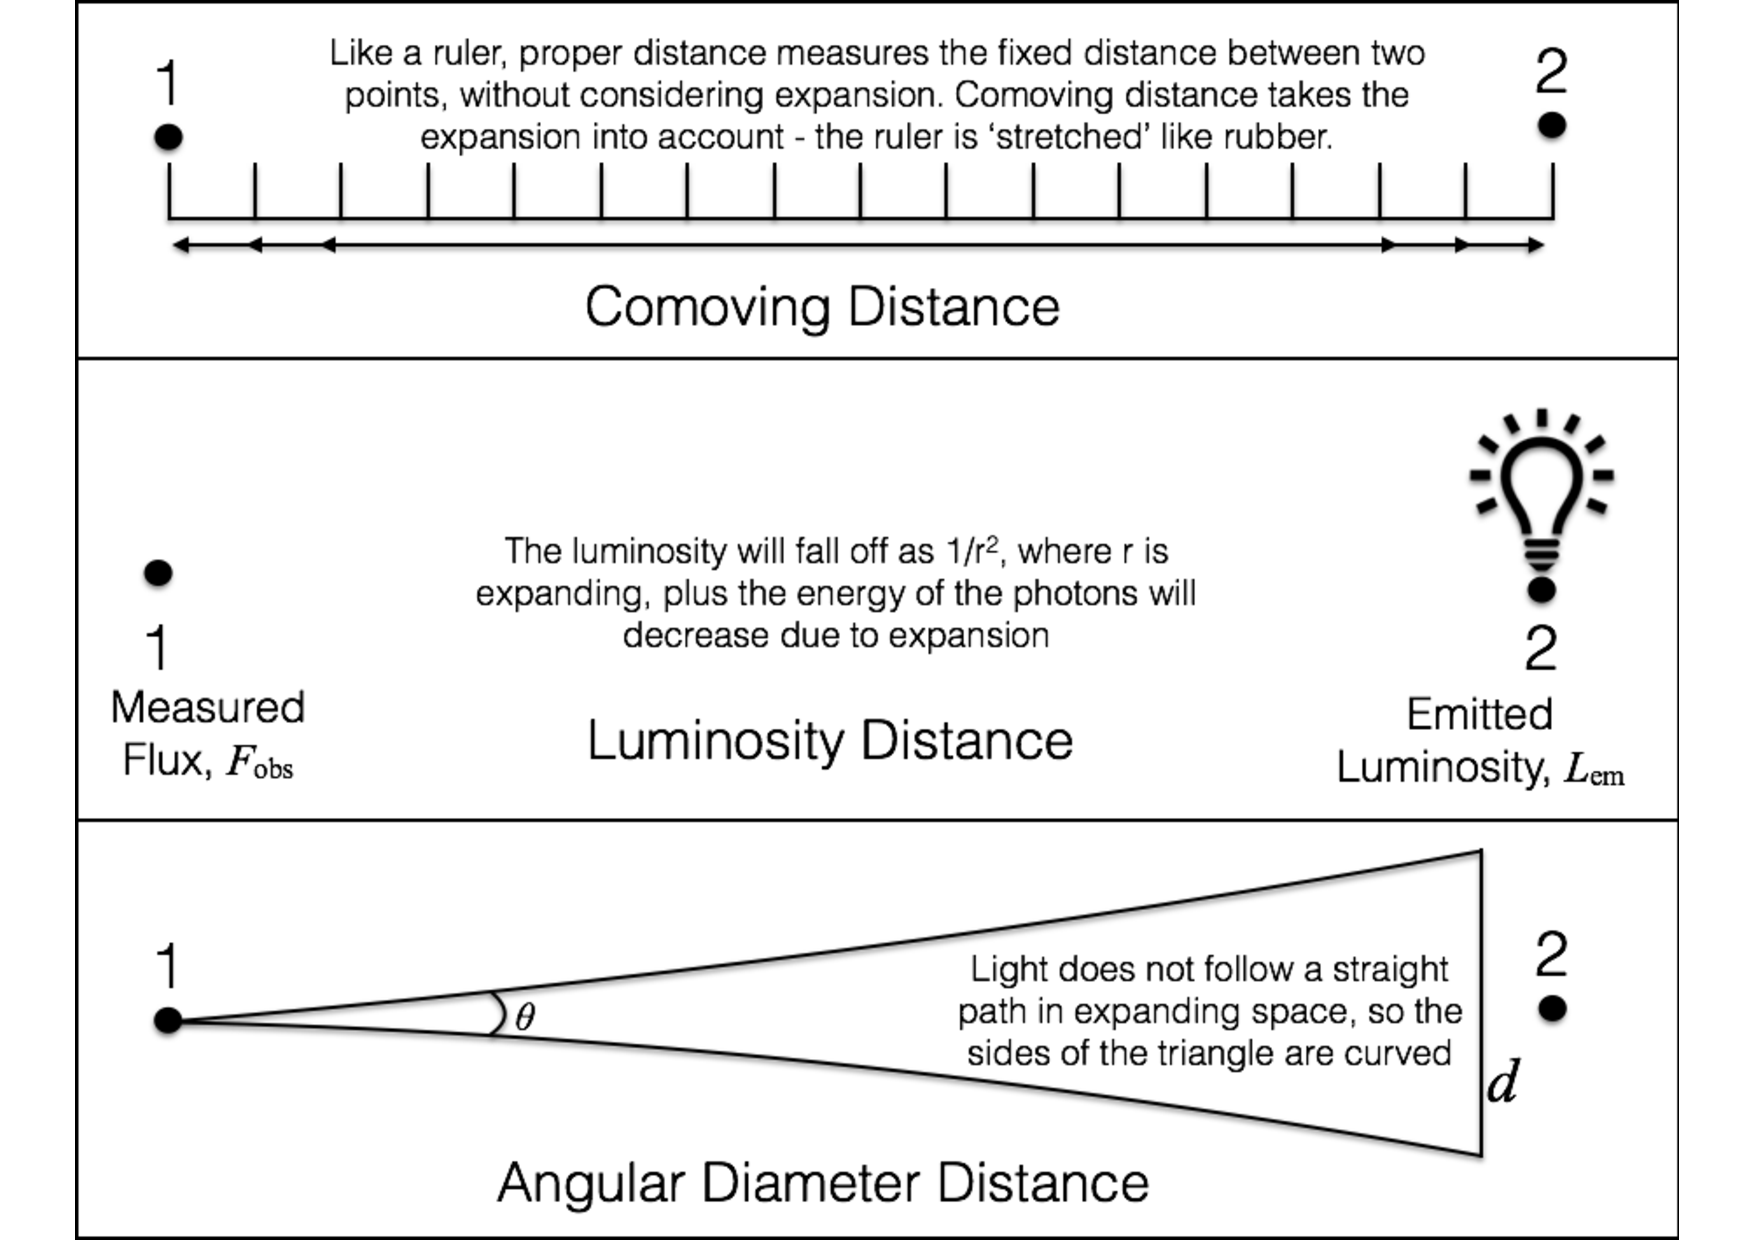
\includegraphics[width=18cm]{Typesofdistances.pdf}
\caption{The three types of distances: Comoving distance, luminosity distance and angular diameter distance.}
\label{fig:distances}
\end{figure*}

\subsection{Age of the universe at redshift z}

The age of the universe at a given redshift can be obtained by integrating up all the time between the beginning of the universe and the time at z. 
\begin{equation}
t_\mathrm{age} = \int_0^{a(t_\mathrm{age})} \frac{\mathrm{d}t}{\mathrm{d}a^\prime} \mathrm{d}a^\prime.
\end{equation}
Now, as mentioned above, the Hubble parameter gives the time rate of change of the scale factor, $a$
\begin{equation}
H = \frac{\dot a}{a} = \frac{\mathrm{d}a}{\mathrm{d}t}\frac{1}{a}.
\end{equation}
Rearranging and substituting into the equation for $t_\mathrm{age}$ gives 
\begin{equation}
\boxed{
\begin{split} 
t_\mathrm{age} = \frac{1}{H_0} &\int_\infty^{z_\mathrm{age}} (1+z)^{-1} H(z) \mathrm{d}z\\
= &\int_\infty^{z_\mathrm{age}} (1+z)^{-1} [\Omega_\mathrm{m} (1+z)^{3}+\Omega_\mathrm{R} (1+z)^{4}+\Omega_\Lambda]^{1/2} \mathrm{d}z
\end{split}
}
\label{eq:tage}
\end{equation}

\section{The code and how to code it}
\label{sec:code}

You are required to write a program which can be run in terminal either like:
\begin{lstlisting}
cdbdmac:cosmology_example Cat$ python cosmo.py --plot_name plot.png --redshift_range -1 4 20
Computing cosmology for:
H_0 = 70.0, Omega_M = 0.3, Omega_L = 0.7
Plotting results, along with some common cosmologies. 
Saving to: `plot.png'
cdbdmac:cosmology_example Cat$
\end{lstlisting}
or like:
\begin{lstlisting}
cdbdmac:cosmology_example Cat$ python cosmo.py --plot_name plot.png --redshift_range -1 4 20 --hubble_const 120 --omega_m 0.01 --omega_L 0.99
Computing cosmology for:
H_0 = 120.0, Omega_M = 0.01, Omega_L = 0.99
Plotting results, along with some common cosmologies. 
Saving to: `plot.png'
cdbdmac:cosmology_example Cat$
\end{lstlisting}
In other words, the inputs \texttt{plot\_name} and \texttt{redshift\_range} are required, and the other inputs are optional. You will need to provide default values for the other inputs in your code (in this case the defaults are \texttt{hubble\_const = 70.0, omega\_m = 0.3, omega\_L = 0.7}). In the above example the redshift range accepts three values: a log-minimum and log-maximum value, and the number of points. A log-spaced set of points is recommended because the behaviour with redshift will be easier to see when you plot it. If you're unsure about this, try starting with linearly spaced redshift points, and change it later.\\

\begin{figure*}[t!]
\makebox[\textwidth][c]{
\includegraphics[width=18cm]{/Users/Caffe/Copy/python_code/cosmology_example/plot.png}
}
\caption{An example output for \texttt{cosmo.py}. The purple line is the user specified input, and is based on the second example input shown above.}
\label{fig:plot.png}
\end{figure*}

\noindent The output of this function should be a plot called `plot.png', which will consist of four panels showing the comoving distance, angular diameter distance, luminosity distance and age at redshift $z$. An example of this plot (corresponding to the second input option above) is shown in Figure~\ref{fig:plot.png}. Note the use of log scales for both the x- and y- axes. You may like to add extra features, such as log scales, titles, a legend, manual line colours, manual axis numbers etc (some of these have been utilised in the plot shown here). \texttt{matplotlib} is as simple or as complicated as you want to make it. If there's something about your plot you want to change, try Googling it and see if you can figure out how. \\

\lstset{frame=tb,
  language=python,
  aboveskip=3mm,
  belowskip=3mm,
  showstringspaces=false,
  columns=flexible,
  basicstyle={\small\ttfamily},
  breaklines=true,
  breakatwhitespace=true,
  tabsize=4
}

\noindent Your program will need to perform the following steps. To create your cosmology calculator, you should aim to complete each of the steps listed below individually, and then join them together only once you have each one working independently and you understand it. You should write all your code into a script (i.e. a .py file), and then run it. Try to avoid coding directly into the interpreter. 

\begin{enumerate}

\item As mentioned above, it must take as its input a plot name, redshift range, and optionally, values of $H_0$, $\Omega_\mathrm{m}$, and/or $\Omega_\mathrm{\Lambda}$ ($\Omega_\mathrm{R}$ is always $0$). To begin with you may want to just hard-code these values and change them in the code each time you want to run it for a different set of values. Once you have everything else working however you should change your code so these are taken as optional arguments in terminal (To do this you want to use the function \texttt{argparse} (Google it!). \itshape{Hint:}\upshape~When using \texttt{argparser} to input the three redshift range values, keep the argument type as \texttt{type=float}, and specify that it can accept multiple values (separated by a space) by adding \texttt{nargs=`+'} to the \texttt{parser.add\_argument()} function call.

\item Use the redshift range to generate a list or array of redshift values. To do this you will want to use either
\begin{enumerate}
\item An inbuilt python \texttt{list}:
\begin{lstlisting}
>>> zmin = 0
>>> zmax = 10
>>> increment = 1
>>> mylist = range(zmin, zmax, increment)
>>> print mylist
[0, 1, 2, 3, 4, 5, 6, 7, 8, 9]
\end{lstlisting}

\item Or a \texttt{numpy} array, with either \texttt{arange()}, \texttt{linspace()}, or \texttt{logspace()}:
\begin{lstlisting}
>>> import numpy as np
>>> zmin = 0
>>> zmax = 10
>>> increment = 1
>>> myarr_1 = np.arange(zmin, zmax, increment)
>>> print myarr_1
[0, 1, 2, 3, 4, 5, 6, 7, 8, 9]
>>> num_pts = 9
>>> myarr_2 = np.linspace(zmin, zmax, num_pts)
>>> print myarr_2
[  0.     1.25   2.5    3.75   5.     6.25   7.5    8.75  10.  ]
>>> logzmin = -2
>>> logzmax = 1
>>> myarr_3 = np.logspace(logzmin,  logzmax, num_pts)
>>> print myarr_3
[  0.01         0.02371374   0.05623413   0.13335214   0.31622777
   0.74989421   1.77827941   4.21696503  10.        ]
\end{lstlisting}
Note that \texttt{arange} does not include the maximum value in the result, whereas \texttt{linspace} and \texttt{logspace} do. 
\end{enumerate}
Again, Google these things to learn about them (including the list comprehension). 

\item Compute the associated cosmological values for each redshift value. This will require performing two numerical integrals for each redshift value, one for the comoving distance, and one for the age of the universe at that redshift. To perform these integrals I recommend using either \texttt{integrate.quad()} from the module \texttt{scipy} or \texttt{quad()} from the module \texttt{mpmath}. Google them to learn about each, and use the one you like the look of! You will probably need to install the \texttt{mpmath} module to use that integrator. You almost certainly already have the \texttt{numpy} and \texttt{scipy} modules with your python installation, but if not you will need to install them. You can iterate over the redshift values a couple of ways:
\begin{enumerate}
\item With a for loop or a while loop:
\begin{lstlisting}
>>> from scipy import integrate
>>> import numpy as np
>>> def f(x, a):
...    return a * x**2
... 
>>> max_xs = np.linspace(1, 10, 5)
>>> a= 1
>>> result = []
>>> for xmax in max_xs:
...     result.append(integrate.quad(f, 0, xmax, args=(a))[0])
...
>>> for xx, res in zip(max_xs, result):
...     print xx, res
... 
1.0 0.333333333333
3.25 11.4427083333
5.5 55.4583333333
7.75 155.161458333
10.0 333.333333333
>>> 
\end{lstlisting}

\item With a list comprehension:
\begin{lstlisting}
>>> from scipy import integrate
>>> import numpy as np
>>> def f(x, a):
...    return a * x**2
... 
>>> max_xs = np.linspace(1, 10, 5)
>>> a = 1
>>> result = [integrate.quad(f, 0, xmax, args=(a))[0] for xmax in max_xs]
>>> for xx, res in zip(max_xs, result):
...     print xx, res
... 
1.0 0.333333333333
3.25 11.4427083333
5.5 55.4583333333
7.75 155.161458333
10.0 333.333333333
>>> 
\end{lstlisting}

\item Or by vectorizing a function with the integral inside it using the \texttt{numpy} function \texttt{vectorize}:
\item With a list comprehension:
\begin{lstlisting}
>>> from scipy import integrate
>>> import numpy as np
>>> def f(x, a):
...    return a * x**2
... 
>>> max_xs = np.linspace(1, 10, 5)
>>> a = 1
>>> def func(xmax, a):
...     return integrate.quad(f, 0, xmax, args=(a))[0]
... 
>>> v_func = np.vectorize(func)
>>> result = v_func(max_xs, a)
>>> for xx, res in zip(max_xs, result):
...     print xx, res
... 
1.0 0.333333333333
3.25 11.4427083333
5.5 55.4583333333
7.75 155.161458333
10.0 333.333333333
>>> 
\end{lstlisting}
\end{enumerate} 
Note that in the above I have used \texttt{scipy.integrate.quad()}. This is a good example for you to build on when writing your own code. 

\item Plot the results of your code for the range of z on a two-by-two set of axes. To do this you will use \texttt{matplotlib.pyplot} and its associated functions. Here is an example of some basic code to make a $4\times 4$ plot with \texttt{matplotlib.pyplot}:
\begin{lstlisting}
>>> import matplotlib.pyplot as plt
>>> import numpy as np
>>> def f(x, a):
...     return a * x**2
...     
>>> x_range = np.linspace(0, 99, 100)
>>> a_vals = [-8, -1, 1, 8]
>>> result = []
>>> for a in a_vals:
...     result.append(f(x_range, a))
>>> # makes the figure, and puts four sets of axes onto it
>>> fig, ((ax1, ax2), (ax3, ax4)) = plt.subplots(2, 2, figsize = (24, 18))
>>> ax1.plot(x_range, result[0])
>>> ax2.plot(x_range, result[1])
>>> ax3.plot(x_range, result[2])
>>> ax4.plot(x_range, result[3])
>>> fig.savefig('myplot.png')
\end{lstlisting}
The Matplotlib website has a extensive set of documentation which you can use to figure out how to build on this. In particular, if you go to the Matplotlib Gallery\footnote{Matplotlib Gallery: http://matplotlib.org/gallery.html}, you can find examples similar to what you want to do, and copy/modify the source code of the example to suit your needs. \\

\end{enumerate}

\noindent The above list is peppered with instructions to Google things. This is because this is $90\%$ of learning python. Any problem you have someone has very likely had before, and they have asked the internet for help. So there's no point in reinventing the wheel - if you have a problem or want to know how to do something, Google it! The best places to look for help or learn how to use a function are the documentation on the module's website (Numpy, Scipy and Matplotlib all have excellent online documentation, as does the core python website), or StackOverflow, an online coding forum. You should check out the function documentation for any function before you use it. \\

\begin{table}[h!]
\caption{Required fundamental constants for writing the code}
\centering
\label{table:constants}
\begin{tabular}{c c c}
\\ [0.05ex]
\hline
\textbf{Constant} & \textbf{Value} & \textbf{Units} \\ [0.5ex]
Speed of light, c & $2.99792458\times 10^5$ & km$\,$s$^{-1}$\\
km in 1 Mpc & $3.08567758147\times 10^{19}$ & km\\
Seconds in 1 year & $3.1557600\times 10^7$ & s\\
\hline
\end{tabular}
\end{table}

\noindent Achieving accurate values for your output requires very accurate input values of the known constants, most of which are hidden in the Hubble constant. In fact, the only units that appear in these calculations are in the Hubble constant, and the speed of light, $c$. The Hubble constant has units km$\,$s$^{-1}$Mpc, and you should use the speed of light in units of km$\,$s$^{-1}$. This will give you distances in units of Mpc. To get the correct value for the age of the universe in years, you need to convert the units of the Hubble constant to be yr$^{-1}$ for use in equation~(\ref{eq:tage}). You can do this by dividing by the number of km in $1$ Mpc and then dividing by the number of seconds in 1 year.  Table~\ref{table:constants} gives the values and units of all the constants required for the code. \\

\noindent You now have all the constants and equations you need for this problem. You also have simple examples of almost all the code you need to construct a basic version of the problem. This code will be much easier to write and follow if you break your code up into different functions, and then put it all together by calling these functions. It will also be a lot easier for you to complete this problem if you attack each of these functions one by one and get each one working before you move onto the next. A suggested structure is:

\begin{itemize}
\item A function for the Friedman Equation (just because it comes up in both integrals). This will look like:
\begin{lstlisting}
def freidman_eq(redshift_z, omega_m, omega_L):
    # The Friedman Eq goes here 
    return freidman_equation_at_redshift_z
\end{lstlisting}

\item Functions for each of the two integrands to be integrated over. These will look like:
\begin{lstlisting}
def an_integrand(redshift_z, omega_m, omega_L):
    # The equation to be integrated goes here.
    # It can be broken up into parts and done over 
    # several lines
    return the_val_of_the_integrand_at_redshift_z
\end{lstlisting}

\item A function to calculate the cosmology for a given set of cosmological parameters. This will contain all the constants (i.e the speed of light and the unit conversions), and will be where you compute the two integrals. You will then use the results of the integrals to compute the comoving distance, angular diameter distance, luminosity distance and age at redshift $z$. This function will look like:
\begin{lstlisting}
def compute_a_cosmol(redshift_z, hubble_const, omega_m, omega_L):
    # The constants get defined here.
    # You also do the integrals, using the functions we just defined above
    # You use the results of these integrals to compute comoving distance, angular diameter distance, luminosity distance 	and age at redshift_z
    return D_c, D_A, D_L, age_at_z
\end{lstlisting}

\item A function to call the \texttt{compute\_a\_cosmol} for the user-specified cosmology, and the three hardcoded ones. All this will need to be fed is the arguments from the \texttt{argparse} function. You might want to start off hardcoding a set of fake `user input' values, get the rest of your code working, then tackle making this function accept the \texttt{argparse} values last. Inside the function you will need to use the redshift range to makes a list of redshifts to compute cosmologies for. You will also need to define a set of lists or dictionaries or something to store the results for each cosmology. You will then call \texttt{compute\_a\_cosmol} for each cosmology, for each redshift value, and store the result in your lists or dictionaries. You will then return them in a list of lists, along with the list of redshift values you used. With \texttt{argparse} in use this function would look like:
\begin{lstlisting}
def compute_all_cosmols(arguments):
    # All the arguments are in `arguments', e.g. H_0 = arguments.hubble_const, Omega_M = arguments.omega_m, max_z, min_z, num_zs = arguments.redshift_range
    # Use the redshift info to make a list or array of redshifts
    # Make some lists or dictionaries to store the results of the calculation for each cosmology
    # For each cosmology, compute the comoving distance, angular diameter distance, luminosity distance and age for each redshift, storing the result in the appropriate list/array
    return list_of_z_vals, [D_c, D_A, D_L, age_at_z] 
\end{lstlisting}
Because of the square brackets around all but the first argument or the return statement, the above function will return two things: a list of redshifts, and a list of lists. Without \texttt{argparse}, this functions can just take the required information as input, e.g \texttt{compute\_all\_cosmols(redshift\_info, H\_0, Omega\_M, Omega\_L)} (remember \texttt{redshift\_info} will be a list of three things: \texttt{max\_z, min\_z and num\_pts}). 

\item A function to plot the results. This will take the name of the output plot image, the list of redshift values the cosmologies were computed for, and the corresponding values of comoving distance, angular diameter distance, luminosity distance and age at redshift $z$ for each cosmology. It's a goo idea to keep all this stuff packed up in lists when you pass it to this function, then unpack it inside the function. This function won't return anything - its job is simply to make a plot and save it. It should look something like:
\begin{lstlisting}
def plot_cosmologies(save_name, list_of_redshifts, list_of_lists_of_cosmologies):
    # Unpack the list_of_lists_of_cosmologies
    # Maka a $4 X 4$ set of axes
    # Plot the comoving distance, angular diameter distance, luminosity distance and age at redshift_z onto the four axes for each cosmology
    # Save the plot to file
    # This function doesn't need a return statement because it doesn't return anything
\end{lstlisting}

\item The argparser. Make this function after you've done everything else. In the mean time, just hardcode some inputs at the top of your script and use them. When you have everything else working have a crack at this. This function takes no arguments, because it gets all its input from the command line. It will look like:
\begin{lstlisting}
def parse_args():
    # Initialise the argparse function as:
    parser = ArgumentParser(description='Cosmology code')
    # Add the command line arguments to parser with: 
    parser.add_argument( stuff.... ) # Remember the plot name and redshift range should be required, everything else should be optional with a default
    # Parse all the arguments provided on the command line with:
    args = parse_args()
    # args now contains all the command line inputs
    return args
\end{lstlisting}

\item Lastly, you need a main function to call all this in. It should look like:
\begin{lstlisting}
def main():
    # Call your argparser first if you've made it. Otherwise, put your `inputs' directly in here
    # Then call your other functions as you need them. You will probably want to call compute_all_cosmols, then plot_cosmologies
    # main doesn't need to return anything
\end{lstlisting}

\item At the end of your script, after \texttt{main()}, add the following so that python knows to call \texttt{main()} by default:
\begin{lstlisting}
if __name__ == '__main__':
    main()
\end{lstlisting}

\end{itemize}

\end{document}



